\PassOptionsToPackage{unicode}{hyperref}
\documentclass[aspectratio=1610, professionalfonts, 9pt]{beamer}

\usefonttheme[onlymath]{serif}
\usetheme[showtotalframes]{tudo}

% Sprachumgebung
\usepackage{polyglossia}
\setmainlanguage{german}

% Mathematik
\usepackage{amsmath}
\usepackage{amssymb}
\usepackage{mathtools}
\usepackage{cancel}

\usepackage[
  math-style=ISO,
  bold-style=ISO,
  sans-style=italic,
  nabla=upright,
  partial=upright,
]{unicode-math}
\setmathfont{Latin Modern Math}

%Links
\usepackage{hyperref}
\usepackage{bookmark}

%%%%%%%%%%%%%%%%%%%%%%%%%%%%%%%%%%%%%%%%%%%%%%%%%%%%%%%%%%%%%%%%%%%%%%%%%%%%%%%%
%%%%%-------------Hier Titel/Autor/Grafik/Lehrstuhl eintragen--------------%%%%%
%%%%%%%%%%%%%%%%%%%%%%%%%%%%%%%%%%%%%%%%%%%%%%%%%%%%%%%%%%%%%%%%%%%%%%%%%%%%%%%%

%Titel:
\title{\LaTeX-Beamer-Theme der TU~Dortmund}
%Autor
\author[M.~Nöthe]{Maximilian Nöthe}
%Lehrstuhl/Fakultät
\institute[Experimental Physics 5]{Names des Lehrstuhls \\  Name der Fakultät}
%Titelgrafik 
\titlegraphic{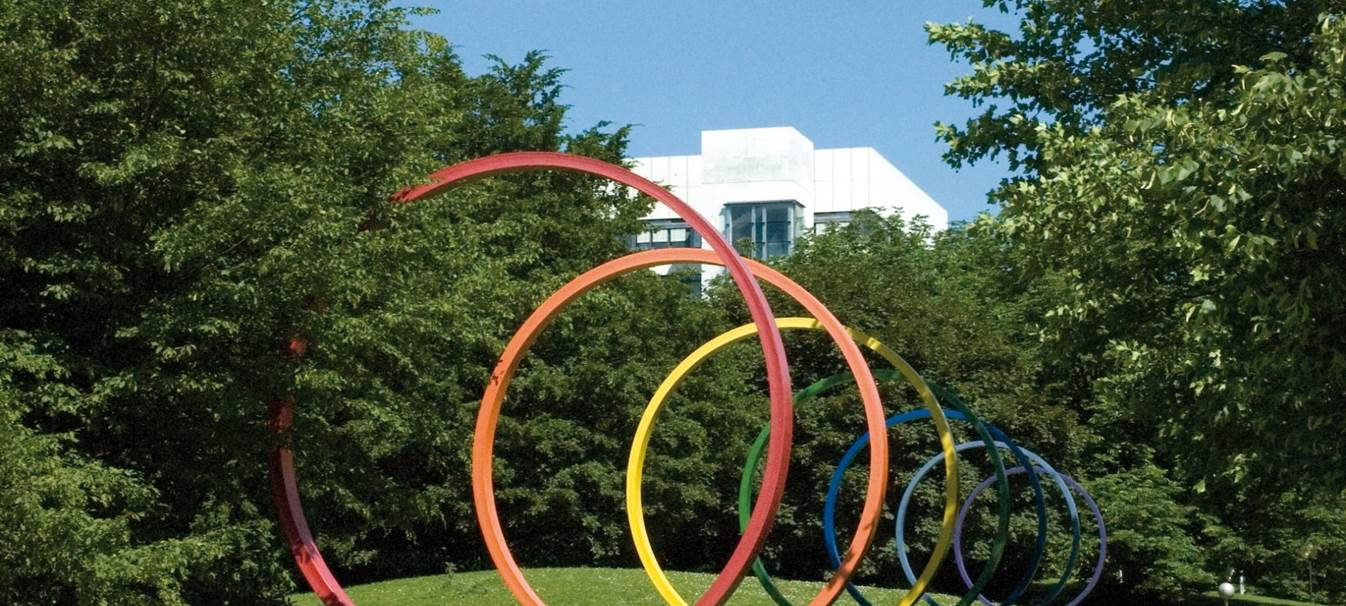
\includegraphics[width=0.7\textwidth]{images/tudo-title-2.jpg}}


\begin{document}

\maketitle

\begin{frame}{Hinweise}
  Zu diesem Theme
  \begin{itemize}
    \item Die .sty-Files müssen im gleichen Verzeichnis wie die .tex liegen
    \item Das Logo in logos/
    \item alternativ können die Dateien an einen beliebigen Ort gelegt werden,
    dies erfordert aber, dass dieser Ordner zu den \texttt{TEXINPUTS} hinzugefügt wird.
  \end{itemize}
  Allgemein zu Beamer und Latex:
  \begin{itemize}
    \item Umfangreicher \LaTeX-Kurs von PeP et Al. \\
      \url{http://toolbox.pep-dortmund.org/notes}
    \item Latex-Beamer Dokumetation:\\
    \url{http://www.ctan.org/pkg/beamer}
  \end{itemize}
\end{frame}

\begin{frame}
    \frametitle{Einführung}
    \tableofcontents[pausesections]
\end{frame}

\section{Blindtext}
\begin{frame}
	\frametitle{Hier steht eine lange, zweizeilige Headline
		\newline gefolgt von einem Blindtext}
Dieser Text dient nur zur Veranschaulichung des Textsatzes. Niemand sollte jemals, aus keinem noch so gutem Grund, so viel Text auf eine Folie packen.

Dies ist ein Blindtext. Dieser Text ist nicht dafür vorgesehen, den Betrachter in die Welt der Dunkelheit zu führen, sondern dafür, einfach etwas Leeres mit etwas Inhaltlosem zu füllen.

Dies ist ein Blindtext. Dieser Text ist nicht dafür vorgesehen, den Betrachter in die Welt der Dunkelheit zu führen, sondern dafür, einfach etwas Leeres mit etwas Inhaltlosem zu füllen.

Dies ist ein Blindtext. Dieser Text ist nicht dafür vorgesehen, den Betrachter in die Welt der Dunkelheit zu führen, sondern dafür, einfach etwas Leeres mit etwas Inhaltlosem zu füllen.

\end{frame}
\end{document}
